%  Copyright 2007-2008 Konrad-Zuse-Zentrum f�r Informationstechnik Berlin
%
%   Licensed under the Apache License, Version 2.0 (the "License");
%   you may not use this file except in compliance with the License.
%   You may obtain a copy of the License at
%
%       http://www.apache.org/licenses/LICENSE-2.0
%
%   Unless required by applicable law or agreed to in writing, software
%   distributed under the License is distributed on an "AS IS" BASIS,
%   WITHOUT WARRANTIES OR CONDITIONS OF ANY KIND, either express or implied.
%   See the License for the specific language governing permissions and
%   limitations under the License.
\documentclass[a4]{scrbook}
\usepackage{typearea}
\areaset[1cm]{165mm}{240mm}

\usepackage[OT1]{fontenc}
\usepackage[latin1]{inputenc}

\usepackage{relsize}
\usepackage{graphicx}
%\usepackage{color}
%\usepackage{colortbl}
\usepackage{makeidx}
\usepackage{fancyhdr}
\usepackage{fancyvrb}
\usepackage{lastpage}
\usepackage{xxcolor}

\usepackage[pdftex,
        colorlinks=true,
        urlcolor=rltblue,       % \href{...}{...} external (URL)
        filecolor=rltblue,     % \href{...} local file
        linkcolor=rltblue,      % \ref{...} and \pageref{...}
%        pagebackref=true,
        pdfborder={0 0 0}]{hyperref}
\usepackage{listings}

\renewcommand{\headrulewidth}{0pt}    % Width of head rule
\renewcommand{\footrulewidth}{0.3pt}  % Width of head rule

% normal pages
\pagestyle{fancy}
\fancyhf{} % clear all header and footer fields
%\fancyhead[RE,LO]{}
\fancyhead[RO]{}%
\fancyfoot[LE,RO]{\bfseries\thepage\ / \pageref{LastPage}}%
\chead{}%
\cfoot{}%

% beginning of a chapter
\fancypagestyle{plain}{%
\fancyhf{} % clear all header and footer fields
%\fancyhead[RE,LO]{}
\fancyhead[RO]{}%
\fancyfoot[LE,RO]{\bfseries\thepage\ / \pageref{LastPage}}%
\chead{}%
\cfoot{}%
}

% Clear Header Style on the Last Empty Odd pages
\makeatletter
\def\cleardoublepage{\clearpage\if@twoside \ifodd\c@page\else%
    \hbox{}%
    \thispagestyle{empty}%              % Empty header styles
    \newpage%
    \if@twocolumn\hbox{}\newpage\fi\fi\fi}
\makeatother

%% Bold typewriter font
\renewcommand{\ttdefault}{pcr}

%%% colors %%%%%%%%%%%%%%%%%%%%%%%%

\definecolor{lightyellow}{rgb}{1.0, 1.0, 0.5}
\definecolor{rltred}{rgb}{0.75,0,0}
\definecolor{rltgreen}{rgb}{0,0.5,0}
\definecolor{rltblue}{rgb}{0,0,0.75}
\definecolor{lightgray}{gray}{0.9}

\setlength{\parindent}{0pt}

\definecolor{lightyellow}{rgb}{1.0, 1.0, 0.5}
\definecolor{codebackground}{rgb}{0.96,0.96,0.8}
\definecolor{commandinput}{rgb}{0.8,0.8,1}

%\thicklines
\lstset{
  basicstyle=\scriptsize\ttfamily,
  backgroundcolor=\color{codebackground},
  keywordstyle=\color{blue}\bfseries,
  % underlined bold black keywords
  identifierstyle=\bfseries, % nothing happens
  commentstyle=\color{red}\bfseries, % white comments
  stringstyle=\sffamily, % typewriter type for strings
  showstringspaces=false,
  xleftmargin=3pt,
  xrightmargin=3pt,
  fancyvrb=true,
  frame=single,
%  frameround=tttt,
%  framexleftmargin=0pt,
  framextopmargin=3pt,
  framexbottommargin=3pt,
%  framexrightmargin=5pt,
  rulecolor=\color{codebackground},
  language=Erlang,
%  fillcolor=\color{red},
%  rulesepcolor=\color{black}
%  rulesep=1cm,
}


\newcommand{\sieheref}[1]{\ref{#1} on page~\pageref{#1}}
\newcommand{\code}[1]{\lstinline[basicstyle=\small\ttfamily]!#1!}
\newcommand{\filetitle}[1]{\hbox to \linewidth{~~File \code{#1:}\hfill}}
\newcommand{\scalaris}{Scalaris}
\newcommand{\todo}[1]{\texttt{\color{red}{#1}}}


\makeindex

\begin{document}
\vspace*{4cm}
\begin{center}
\setlength{\parskip}{0.8cm}
{
\Huge
\bf \textit{\it\sffamily Scalaris}

 \textsf{Users and Developers Guide}

\textsf{Version 0.1}
}

{\LARGE Florian Schintke, Thorsten Sch�tt}

{\LARGE \today}
\vfill
\end{center}
\pagebreak
\mbox{}
\vfill

Copyright 2007-2008 Konrad-Zuse-Zentrum f�r Informationstechnik Berlin

\medskip
Licensed under the Apache License, Version 2.0 (the "License");
you may not use this file except in compliance with the License.
You may obtain a copy of the License at

\medskip
\url{http://www.apache.org/licenses/LICENSE-2.0}

\medskip
Unless required by applicable law or agreed to in writing, software
distributed under the License is distributed on an "AS IS" BASIS,
WITHOUT WARRANTIES OR CONDITIONS OF ANY KIND, either express or implied.
See the License for the specific language governing permissions and
limitations under the License.

\tableofcontents

\part{Users Guide}

\chapter{Download and Installation}

\section{Requirements}

For building and running \scalaris{}, some third-party modules are
required which are not included in the \scalaris{} sources:

\begin{itemize}
\setlength{\itemsep}{0pt}
\setlength{\parskip}{0pt}
\item Erlang R12
\item Erlang OTP (included in Erlang R12)
\item Erlang yaws
\item GNU Make
\item rrdtool
\end{itemize}

Note, the Version 12 of Erlang is required. \scalaris{} will not
work with older versions.

To build the Java API the following modules are required additionally:

\begin{itemize}
\setlength{\itemsep}{0pt}
\setlength{\parskip}{0pt}
\item Java Development Kit 1.6
\item Apache Ant
\end{itemize}

Before building the Java API, make sure that \code{JAVA\_HOME} and
\code{ANT\_HOME} are set. \code{JAVA\_HOME} has to point to a JDK
1.6 installation, and \code{ANT\_HOME} has to point to an Ant
installation.

\section{Download}

The sources can be obtained from \url{http://code.google.com/p/scalaris}.

\subsection{Development Branch}

You find the latest development version in the svn repository:
\begin{lstlisting}[language=sh]
# Non-members may check out a read-only working copy anonymously over HTTP.
svn checkout http://scalaris.googlecode.com/svn/trunk/ scalaris-read-only
\end{lstlisting}

\subsection{Releases}

Releases can be found under the 'Download' tab on the web-page.


\section{Configuration}

\scalaris{} reads the two configuration files from the working directory:
\code{bin/scalaris.cfg} (mandatory) and \code{bin/scalaris.local.cfg}
(optional). The former defines default settings and is included in the
release. The latter can be created by the user to alter settings.  A sample
file is \code{bin/scalaris.local.cfg.example}. A local configuration file is
necessary to run \scalaris{} on distributed nodes:

\begin{lstlisting}[title=\filetitle{scalaris.local.cfg}]
% Insert the appropriate IP-addresses for your setup as comma separated integers.
% IP Address, Port, and label of the boot server
{boot_host, {{209,85,135,99},14195,boot}}.

% IP Address, Port, and label of the log server
{log_host, {{209,85,135,99},14195,boot_logger}}.

% possible values: 14195, [14195, 14196, 14197] (list of ports), 
% or {14195, 15000} as range of ports
{listen_port, 14195}.
\end{lstlisting}

\code{boot_host} defines the node where the boot server is running, which is
contacted to join the system.

\section{Build}

%\subsection{Windows (Win32)}
% \begin{enumerate}
% \setlength{\itemsep}{0pt}
% \setlength{\parskip}{0pt}
% \item Copy \code{make.exe} from \code{contrib/win32} to \code{src} 
% \item Copy \code{Makefile_to_src} from \code{contrib/win32} to \code{src} 
% \item Copy \code{Makefile_to_src_comm_layer} from \code{contrib/win32} to \code{src/comm_layer} 
% \item Copy \code{Makefile_to_src_transstore} from \code{contrib/win32} to \code{src/transstore} 
% \item Rename Makefiles
% \item Open MS-DOS Command Shell 
% \item Go into \code{src} directory 
% \item Call \code{make}
% \item Go into bin directory 
% \item Call \code{boot.bat}
% \end{enumerate}
% 
% \subsubsection{Troubleshooting}
% Check path to Erlang Installation in Makefiles.

\subsection{Linux}

Read the file \code{README} in the main \scalaris{} checkout directory.

\subsection{Java-API}

The following commands will build the Java API for \scalaris{}:
\begin{lstlisting}[language=sh]
%> cd java-api
%> ant 
\end{lstlisting}

This will build chordsharp4j.jar, which is the library for accessing
the overlay network. Optionally, the documentation can be build:
\begin{lstlisting}[language=sh]
%> ant doc
\end{lstlisting}


\section{Running \scalaris{}}

In \scalaris{} there are two kinds of processes:
\begin{itemize}
\setlength{\itemsep}{0pt}
\setlength{\parskip}{0pt}
\item boot servers
\item regular servers
\end{itemize}

In every \scalaris{}, at least one boot server is required. It will
maintain a list of nodes taken part in the system and allows other
nodes to join the ring. For redundancy, it is also possible to have
several boot servers.

\subsection{Running on a local machine}
\label{sec.boot}

Open at least two shells. In the first, go into the bin directory:
\begin{lstlisting}[language=sh]
%> cd bin
%> ./boot.sh
\end{lstlisting}

This will start the boot server. On success \url{http://localhost:8000}
should point to the management interface page of the boot server. The main
page will show you the number of nodes currently in the system. After a
couple of seconds a first \scalaris{} should have started in the boot server
and the number should increase to one. The main page will also allow you to
store and retrieve key-value pairs.

The boot server should show output similar to the following, when
starting the first \scalaris{} nodes. The first line is printed when
the \scalaris{} is spawned. Afterwards it will try to connect the
boot server. When the third line is printed, it managed to contact the
boot server and joined the ring. In this case, it was the first node
in the ring.
\begin{lstlisting}
[ I | Node   | <0.97.0> ] joining "23947834870"
[ I | Node   | <0.97.0> ] join as first [50,51,57,52,55,56,51,52,56,55,48]
[ I | Node   | <0.97.0> ] joined
\end{lstlisting}

In a second shell, you can now start a second \scalaris{} node. This
will be a `regular server'. Go in the bin directory:
\begin{lstlisting}[language=sh]
%> cd bin
%> ./cs_local.sh
\end{lstlisting}

The second node will read the configuration file and use this
information to contact the boot server and will join the ring. The
number of nodes on the web page should have increased to two by now.

Optionally, a third and fourth node can be started on the same
machine. In a third shell:
\begin{lstlisting}[language=sh]
%> cd bin
%> ./cs_local2.sh
\end{lstlisting}


In a fourth shell:
\begin{lstlisting}[language=sh]
%> cd bin
%> ./cs_local3.sh
\end{lstlisting}


This will add 3 nodes to the network. The web pages at
\url{http://localhost:8000} should show the additional nodes.

\subsection{Running distributed}

\scalaris{} can be installed on other machines in the same way as described
in Sect.~\ref{sec:install}. Please make sure, that the
\code{scalaris.local.cfg} refers to available boot servers. Otherwise the
other nodes will not find the boot server. On the remote nodes, you only
need to call \code{./cs_local.sh} and they will automatically contact the
configured boot server.

\subsection{Running on PlanetLab}

\subsection{Replication Degree}

\subsection{Routing Scheme}

\section{Installation}

Note: there is no \code{make install} at the moment! The nodes have
to be started from the bin directory.




\chapter{Using the system}

\section{Erlang}

\section{Java command line interface}

The jar file contains a small command line interface client.

\begin{lstlisting}[language=sh]
%> java -jar chordsharp4j.jar -help
usage: chordsharp
 -getsubscribers <topic>   get subscribers of a topic
 -help                     print this message
 -publish <params>         publish a new message for a topic: <topic>
                           <message>
 -read <key>               read an item
 -subscribe <params>       subscribe to a topic: <topic> <url>
 -write <params>           write an item: <key> <value>
\end{lstlisting}

Read and write can be used to read resp. write from/to the
overlay. getsubscribers, publish, and subscribe are the PubSub
functions.

\begin{lstlisting}[language=sh]
%> java -jar chordsharp4j.jar -write foo bar
write(foo, bar)
%> java -jar chordsharp4j.jar -read foo
read(foo) == bar
\end{lstlisting}

The chordsharp4j library requires that you are running a `regular server' on
the same node. Having a boot server running on the same node is not
sufficient.

\section{Java API}

\chapter{Testing the system}

\section{Running the unit tests}
There are some unit tests in the \code{test} directory. You can call them
by running \code{make test} in the main directory. The results are stored
in a local \code{index.html} file. The tests use the \code{common-test}
package from the Erlang system. 

\part{Developers Guide}

\chapter{How a node joins the system}

\hfill\emph{2008-07-22, SVN revision 2}

\section{General Erlang server loop}

Servers in Erlang often use the following structure to maintain a state
while processing received messages:

\lstset{language=Erlang}
\begin{lstlisting}%[title=\filetitle{foo.erl}]
loop(State) ->
  receive
    Message ->
      State1 = f(State),
      loop(State1)
  end.
\end{lstlisting}

The server runs an endless loop, that waits for a message, processes it and
calls itself using tail-recursion in each branch. The loop works on a
\code{State}, which can be modified when a message is handled.

\section{Starting additional local nodes after boot}

After booting a new \scalaris-System as described in
Section~\sieheref{sec.boot}, ten additional local nodes can be started
by typing \code{admin:add_nodes(10)} in the Erlang-Shell that the boot
process opened.


\lstset{language=Erlang}
\begin{lstlisting}
scalaris/bin> ./boot.sh
[...]
=INFO REPORT==== 18-Jul-2008::20:08:48 ===
Yaws: Listening to 0.0.0.0:8000 for servers
 - http://localhost:8000 under ../docroot
[ I | Fail   | <0.102.0> ] start detector
this() == {{127,0,0,1},14195}
[ I | Node   | <0.105.0> ] joining "22500913918"
[ I | Node   | <0.105.0> ] join as first [50,50,53,48,48,57,49,51,57,49,56]
[ I | Node   | <0.105.0> ] joined

(boot@csr-pc9)1> admin:add_nodes(10)
\end{lstlisting}

In the following we will trace, what this function does to join
additional nodes to the system.

The function \code{admin:add_nodes(int)} is defined as follows.
\begin{lstlisting}[title=\filetitle{admin.erl}]
[...]
add_nodes(Count) ->
    randoms:init(),
    add_nodes_loop(Count).

add_nodes_loop(0) ->
    ok;
add_nodes_loop(Count) ->
    io:format("~p~n", [supervisor:start_child(main_sup, {randoms:getRandomId(),
                                                        {cs_sup_or, start_link, []},
                                                        permanent,
                                                        brutal_kill,
                                                        worker,
                                                        []})]),
    add_nodes_loop(Count - 1).
[...]
\end{lstlisting}

It first initializes the random number generator and then calls
\code{add_nodes_loop(Count)}.

This function starts a new child for the main supervisor \code{main_sup}.
As defined by the parameters, to actually perform the start, the function
\code{cs_sup_or:start_link} is called by the Erlang supervisor mechanism.
For more details on the OTP supervisor mechanism see Chapter 18 of the
Erlang book~\cite{erlang-book} or the online documentation at 
\url{http://www.erlang.org/doc/man/supervisor.html}.

\subsection{Supervisor-tree of a \scalaris{} node}

When starting a new node in the system, the following supervisor tree is
created:

\medskip
{\centering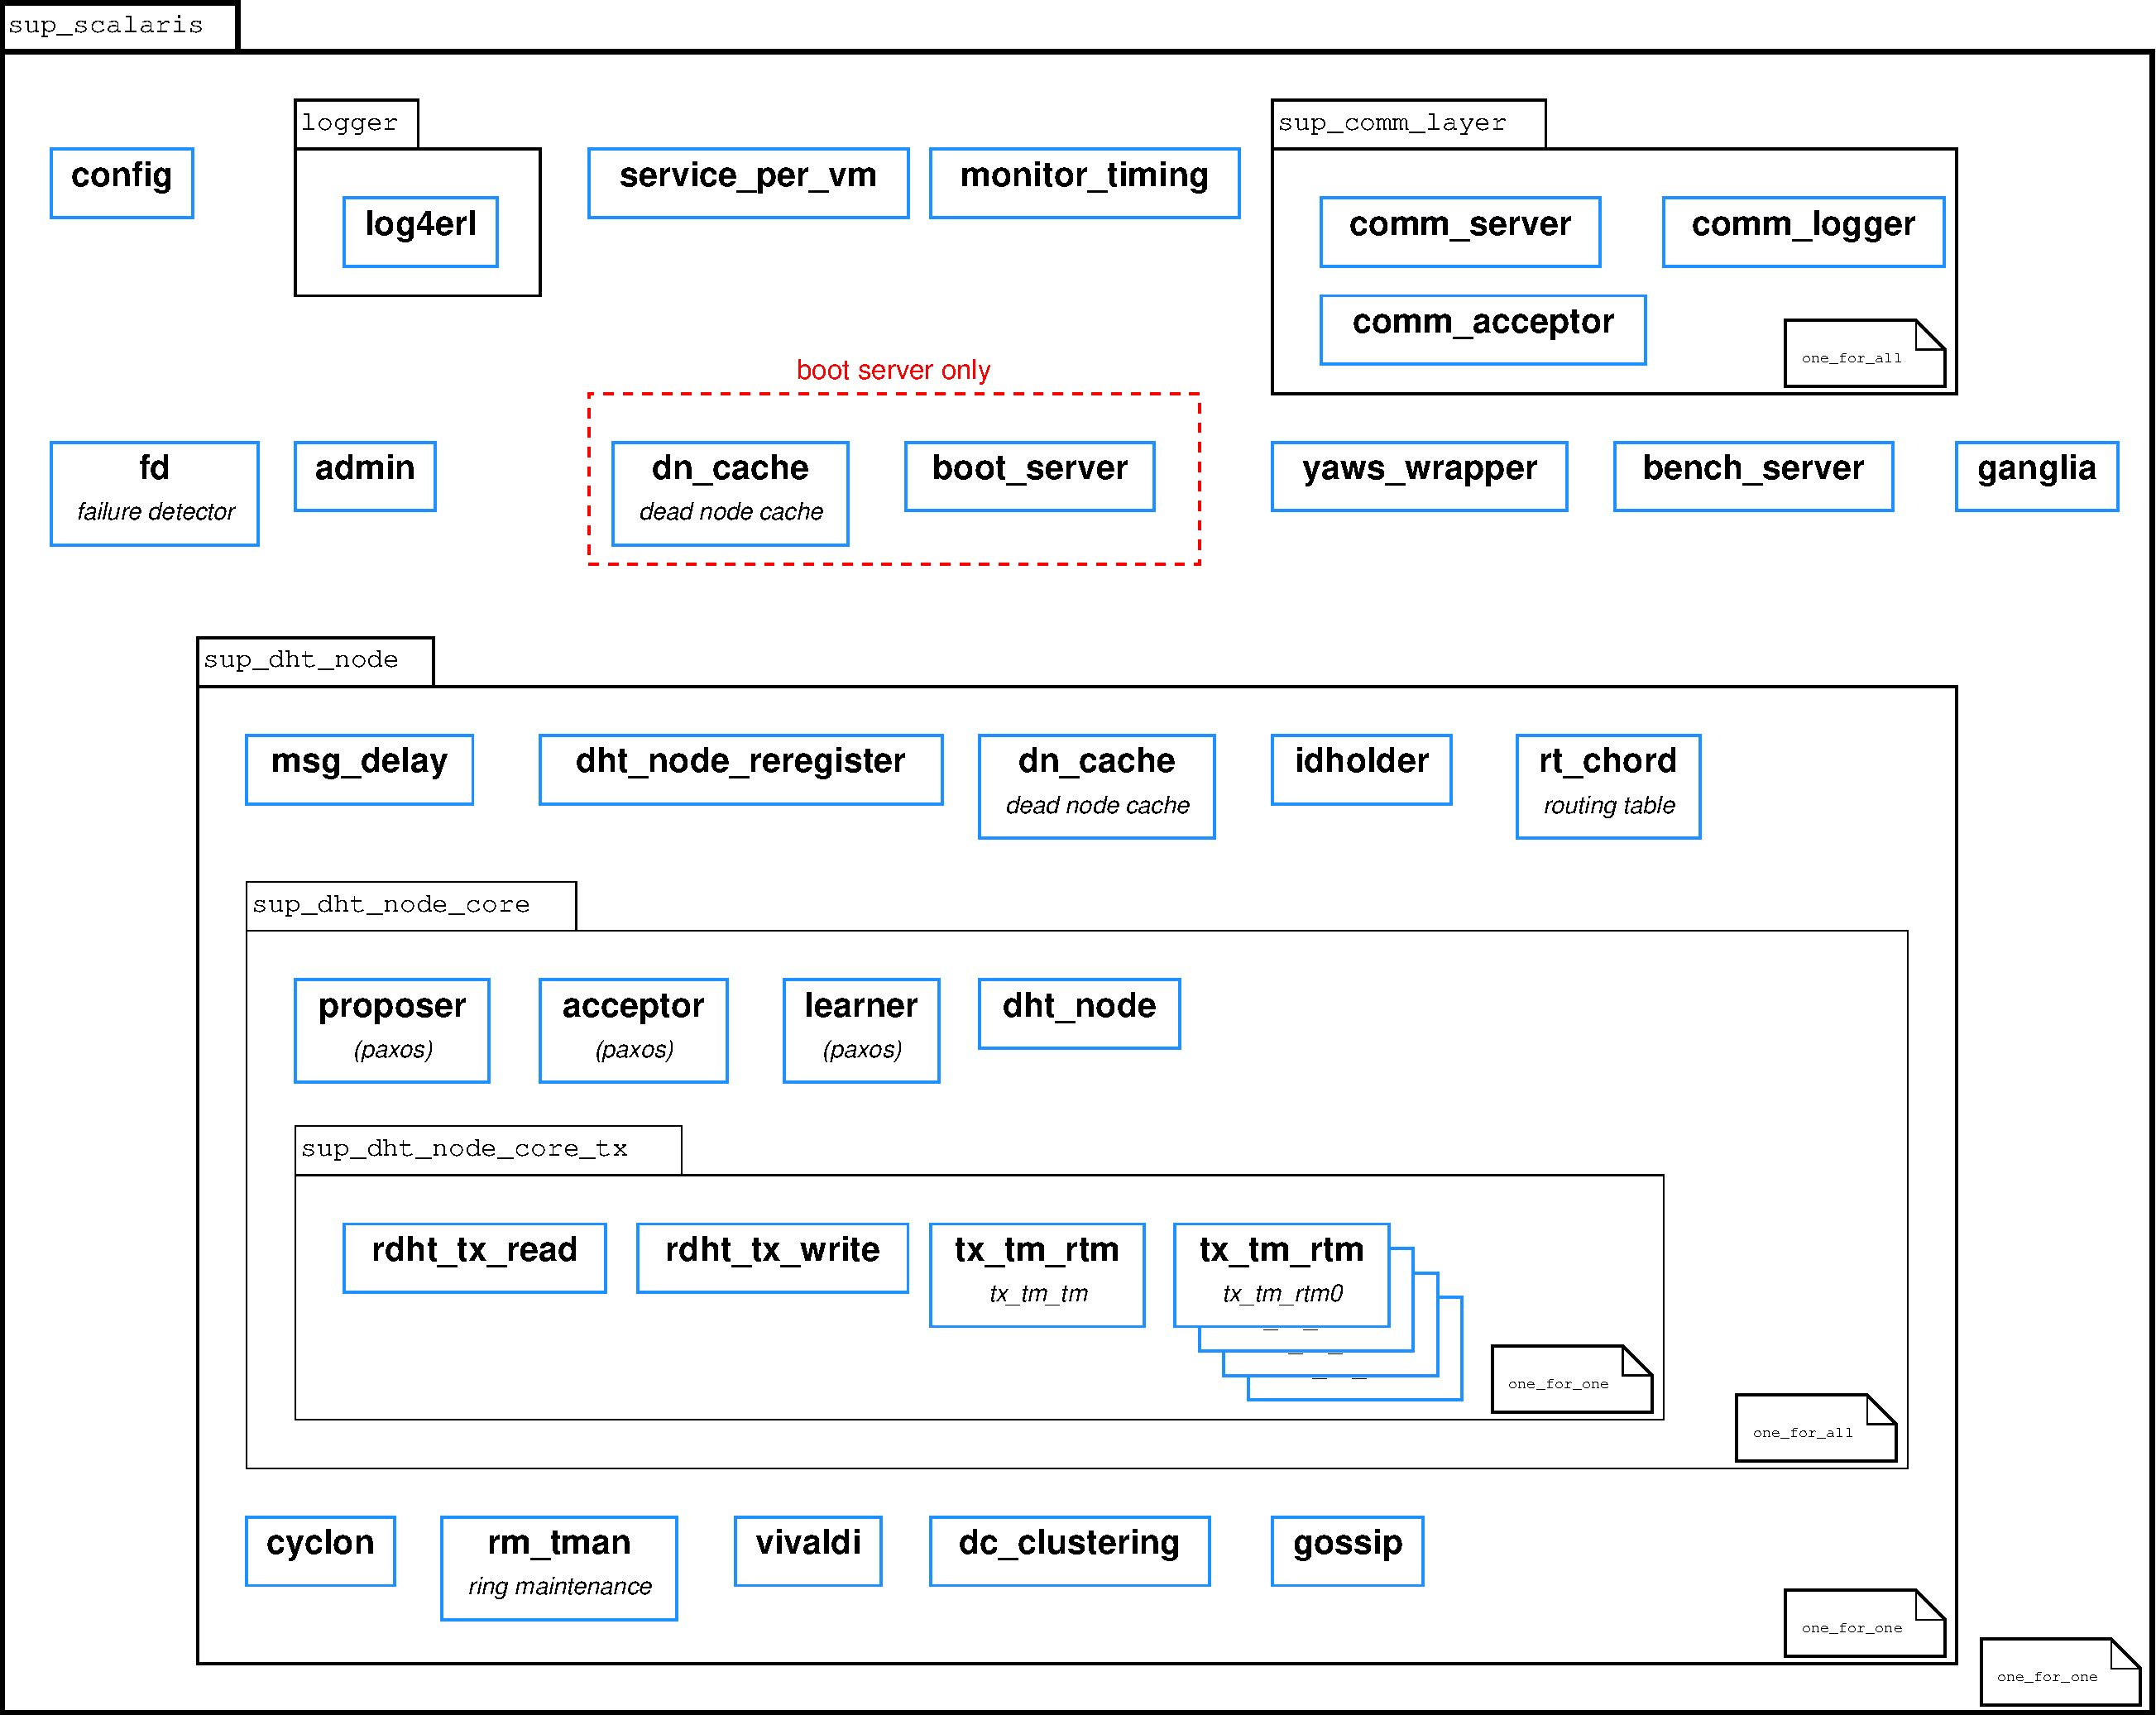
\includegraphics[width=0.9\linewidth]{supervision}}

\subsection{Starting the or-supervisor and general processes of a node}

The supervisor mechanism first calls the \code{init()} function of the
defined module (\code{cs_sup_or:init()} in this case) before calling the
defined start function (\code{start_link} here.

So, lets have a look at \code{cs_sup_or:init}, the 'Scalaris
\emph{or} supervisor'.
 
\begin{lstlisting}[title=\filetitle{cs_sup_or.erl}]
[...]
init([]) ->
    randoms:init(),
    InstanceId = string:concat("cs_node_", randoms:getRandomId()),
    FailureDetector =
	{failure_detector,
	 {failuredetector, start_link, [InstanceId]},
	 permanent, brutal_kill, worker,
	 [failure_detector]
     },
    KeyHolder =
	{cs_keyholder,
	 {cs_keyholder, start_link, [InstanceId]},
	 permanent, brutal_kill, worker,
	 []},
    MessageStatisticsCollector = 
	{cs_message_collector,
	 {cs_message, start_link, [InstanceId]},
	 permanent, brutal_kill, worker,
	 []},
    Supervisor_AND = 
	{cs_supervisor_and,
	 {cs_sup_and, start_link, [InstanceId]},
	 permanent, brutal_kill, supervisor,
	 []},
    {ok, {{one_for_one, 10, 1},
	  [
	   KeyHolder,
	   MessageStatisticsCollector,
	   FailureDetector,
	   Supervisor_AND
	  ]}}.
[...]
\end{lstlisting}

The \code{init()} function must return process descriptions that the
supervisor should start, and how the processes have to be observed. Here, we
define a list of processes to be observed by a \code{one_for_one}
supervisor. The processes are: \code{Config}, \code{KeyHolder},
\code{MessageStatisticsCollector} and a \code{Supervisor_AND} process.

The term \code{\{one_for_one, 10, 1\}} defines that the supervisor should
  retry 10 times to restart each process before giving
  up. \code{one_for_one} supervision means, that if a single process stops,
  only that process is restarted. The other processes run independently.

The \code{cs_sup_or:init()} is finished and the supervisor
module, starts all the defined processes by calling their corresponding
\code{init()} functions and afterwards, the functions that were defined in
the list of the \code{cs_sup_or:init()}.

For a join of a new node, we are only interested in the starting of the
\code{Supervisor_AND} process here, which was the last one in the list. At
that point in time, all other defined processes are already started and
running.

\subsection{Starting the and-supervisor with a peer and its local database}

Again, the OTP will first call the \code{init()} function of the
corresponding module:

\begin{lstlisting}[title=\filetitle{cs_sup_and.erl}]
[...]
init([InstanceId]) ->
    Node =
	{cs_node,
	 {cs_node, start_link, [InstanceId]},
	 permanent,
	 brutal_kill,
	 worker,
	 []},
    DB =
	{cs_db_otp,
	 {cs_db_otp, start_link, [InstanceId]},
	 permanent,
	 brutal_kill,
	 worker,
	 []},
    {ok, {{one_for_all, 10, 1},
	  [
	   DB,
	   Node
	  ]}}.
[...]
\end{lstlisting}

It defines two processes, that have to be observed using an
\code{one_for_all}-supervisor, which means, that if one fails, all have to
be restarted. Passed to the \code{init} function is the \code{InstanceId}, a
random number to make nodes unique. It was calculated a bit earlier in
the code. Exercise: Try to find where.

As you can see from the list, the \code{DB} is started before the
\code{Node}. This is intended and important, because \code{cs_node} uses the
database, but not vice versa.

After the \code{cs_sup_and:init()} finished, the DB is initialized and
afterwards \code{cs_node:start_link} is called by the and-supervisor.
We only go into details here, for the latter.

\begin{lstlisting}[title=\filetitle{cs_node.erl}]
[...]
start_link(InstanceId) ->
    {ok, spawn_link(?MODULE, start, [InstanceId])}.
[...]
\end{lstlisting}

This spawns a new process, that executes \code{cs_node:start()} and
maintains a link to that process. This function is called in the context of
the and-supervisor process, so the and-supervisor process will be informed,
when the spawned process finishes. After the spawn is submitted,
\code{cs_node:start_link} returns to the supervisor, which starts observing
the processes in a loop.

Note: \code{?MODULE} is a predefined Erlang macro, which expands to the
module name, the code belongs to (here: \code{cs_node}).

\subsection{Initializing a \code{cs_node}-process}

\begin{lstlisting}[title=\filetitle{cs_node.erl}]
[...]
start(InstanceId) ->
    %register(cs_node, self()),
    process_dictionary:register_process(InstanceId, cs_node, self()),
    randoms:init(),
    timer:sleep(random:uniform(100) * 100),
    Id = cs_keyholder:get_key(),
    failuredetector:set_owner(self()),
    boot_server:connect(),
    {First, State} = cs_join:join(Id),
    if
	not First ->
	    cs_replica_stabilization:recreate_replicas(
              cs_state:get_my_range(State));
	true ->
	    ok
    end,
    timer:send_after(config:stabilizationInterval(), 
      self(), {stabilize_ring}),
    timer:send_after(config:pointerStabilizationInterval(),
      self(), {stabilize_pointers}),
    timer:send_after(config:failureDetectorUpdateInterval(),
      self(), {stabilize_failuredetector}),
    timer:send_after(config:loadBalanceStartupInterval(),
      self(), {stabilize_loadbalance}),
    io:format("[ I | Node   | ~w ] joined~n",[self()]),
    loop(State, cs_debug:new()).
[...]
\end{lstlisting}

A \code{cs_node} first registers itself in the process dictionary.  Then,
the process sleeps for a random amount of time. Otherwise, if you would
start 1000 processes with \code{admin:add_nodes(1000)}, the boot-server
would receive many join requests at the same time, which is not intended.

Then, the node retrieves its \code{Id} from the keyholder: \code{Id =
  cs_keyholder:get_key()}. In the first call, a random identifier is
returned, otherwise the latest set value. If the \code{cs_node}-process
failed and is restarted by its supervisor, this call to the keyholder
ensures, that the node still keeps its \code{Id}, assuming that the
keyholder process is not failing.  This is important for the load-balancing
and for consistent responsibility of nodes to ensure consistent lookup in
the structured overlay. Note: the name \code{Key-holder} actually is an
id-holder.

If a node changes its position in the ring for load-balancing, the
key-holder will be informed and the \code{cs_node} finishes itself. This
triggers a restart of the corresponding database process via the
and-supervisor.  When the supervisor restarts both processes, they will
retrieve the new position in the ring from the key-holder and join the ring
there.

\todo{The supervisor was configured to restart a node at most 10 times. Does
  that mean, that a node can only change its position in the ring 10 times
  (caused by load-balancing)?}

Next, the \code{cs_node} registers itself as the owner of the
failuredetector \code{failuredetector:set_owner(self())} to become informed,
when the failuredetector detects failing nodes.

With \code{boot_server:connect()} a connection to the boot-server is
established.

\subsection{Actually joining the ring}

\code{cs_join:join} is called next in \code{cs_node:start()}.

\begin{lstlisting}[title=\filetitle{cs_join.erl}]
[...]
join(Id) -> 
    io:format("[ I | Node   | ~w ] joining ~p ~n",[self(), Id]),
    Ringsize = boot_server:number_of_nodes(),
    if
	Ringsize == 0 ->
	    State = join_first(Id),
	    cs_reregister:reregister(cs_state:uniqueId(State)),
	    {true, State};
	true ->
	    case cs_lookup:reliable_get_node(erlang:get(instance_id), 
					     Id, 60000) of
		error ->
		    join(Id);
		{ok, Succ} ->
		    State = join_ring(Id, Succ),
		    cs_reregister:reregister(cs_state:uniqueId(State)),
		    {false, State}
	    end
    end.
[...]
\end{lstlisting}

The boot-server is contacted to retrieve the known number of nodes in the
ring. If the ring is empty, \code{join_first} is called. Otherwise,
\code{join_ring} is called.

\code{join_first} just creates a new state for a \scalaris{} node consisting
of an empty routing table, a successorlist containing itself, itself as its
predecessor, a reference to itself, its responsibility area from \code{Id}
to \code{Id} (the full ring), and a load balancing schema.

\begin{lstlisting}[title=\filetitle{cs_join.erl}]
[...]
join_first(Id) -> 
    io:format("[ I | Node   | ~w ] join as first ~w ~n",[self(), Id]),
    Me = node:make(cs_send:this(), Id),
    cs_state:new(?RT:empty(Me), [Me], Me, Me, {Id, Id}, cs_lb:new()).
\end{lstlisting}

The macro \code{?RT} maps to the configured routing algorithm. It is defined
in \code{chordsharp.erl}. For further details on the routing see Chapter~\sieheref{chapter.routing}.

The state is defined in 

\begin{lstlisting}[title=\filetitle{cs_state.erl}]
[...]
new(RT, SuccessorList, Predecessor, Me, MyRange, LB) ->
    #state{
     routingtable = RT,
     successorlist = SuccessorList,
     predecessor = Predecessor,
     me = Me,
     my_range = MyRange,
     lb=LB,
     join_time=now(),
     deadnodes = gb_sets:new(),
     trans_log = #translog{
       tid_tm_mapping = dict:new(),
       decided = gb_trees:empty(),
       undecided = gb_trees:empty()
      }
    }.
[...]
\end{lstlisting}

If a node joins an existing ring, \code{reliable_get_node} for the own
\code{Id} is called in \code{cs_join:join()}. This lookup delivers the
successor for the joining node. The node, that is currently responsible for
\code{Id}, but which has a larger \code{Id} itself.  If this lookup fails
for some reason, it is tried again, by recursivly calling the \code{join()}.

\todo{What, if the \code{Id} is exactly the same as that of the existing
  node? This could lead to lookup and responsibility inconsistency? Can this
  be triggered by the load-balancing? This is a bug, that should be
  fixed!!!}

Then, \code{cs_join:join_ring} is called:

\begin{lstlisting}[title=\filetitle{cs_join.erl}]
[...]
join_ring(Id, Succ) ->
    io:format("[ I | Node   | ~w ] join_ring ~w ~n",[self(), Id]),
    Me = node:make(cs_send:this(), Id),
    UniqueId = node:uniqueId(Me),
    cs_send:send(node:pidX(Succ), {join, cs_send:this(), Id, UniqueId}),
    receive
	{join_response, Pred, Data, SuccList} -> 
	    io:format("[ I | Node   | ~w ] got pred ~w~n",[self(), Pred]),
	    IsNull = node:is_null(Pred),
	    if
		IsNull ->
		    failuredetector:add_node(node:uniqueId(Succ), 
                      node:id(Succ), node:pidX(Succ));
		true ->
		    failuredetector:add_nodes([{node:uniqueId(Pred), 
                      node:id(Pred), node:pidX(Pred)}, 
	              {node:uniqueId(Succ), node:id(Succ), node:pidX(Succ)}]),
		    cs_send:send(node:pidX(Pred), {update_succ, Me})
	    end,
	    cs_db_otp:add_data(Data),
	    cs_state:new(?RT:empty(Succ), [Succ | SuccList], Pred, Me, 
              {node:id(Pred), Id}, cs_lb:new())
    end.
[...]
\end{lstlisting}

First the node is initialized. Then it sends a \code{join} message to the
successor including a reference to itself and the chosen \code{Id}.

The message is received by the old node in \code{cs_node.erl}. There exists
a \code{\{join, X\}} handler. 

\begin{lstlisting}[title=\filetitle{cs_node.erl}]
[...]
  {join, Source_PID, Id, UniqueId} = _Message -> 
    ?LOG("[ ~w | I | Node   | ~w ] join~n",
	      [calendar:universal_time(), self()]),
    NewState = cs_join:join_request(State, Source_PID, Id, UniqueId),
    loop(NewState, ?DEBUG(cs_debug:debug(Debug, NewState, _Message)));
[...]
\end{lstlisting}

This triggers to call \code{join_request} on the old node. 

\begin{lstlisting}[title=\filetitle{cs_join.erl}]
[...]
join_request(State, Source_PID, Id, UniqueId) ->
    Pred = node:new(Source_PID, Id, UniqueId),
    HisData = cs_db_otp:split_data(State, Id),
    SuccList = cs_state:succ_list(State),
    cs_send:send(Source_PID, {join_response, cs_state:pred(State), HisData, SuccList}),
    failuredetector:add_node(UniqueId, Id, Source_PID),
    cs_state:update_pred(State, Pred).
[...]
\end{lstlisting}

This resets the local predecessor to the new node and splits the data.
Then it sends a \code{join_response} to the new node with its former
predecessor, the data, it has to host, and its successorlist.
Additionally, the new node will be observed by the failuredetector.

Note: Here, the observation of the former predecessor could be deleted from
the failure detector. But periodically, all known hosts are reregistered
with the failure detector, and then all other nodes are thrown away from the
list of nodes to observe in the failure detector. So, we do not care here.

Finally, the new predecessor is set and the \code{join_request()} is finished.
 
Back on the new node: it waits for the \code{join_response} message in
\code{cs_join:join_ring()}. The next steps after the message was received
from the old node are to register the predecessor, to register all new nodes
in the failure detector, to send a message to the predecessor, that its
successor has changed.

Finally, all data are added to the database and the succlist is build by
putting the successor to the head of the successor list of the successor
(old node): \code{[Succ | SuccList]}.

The next step in \code{cs_join:join()} is to call
\code{cs_reregister:reregister} which reregisters the node periodically with
the boot server. Then \code{\{false, State\}} is returned, which means 'this
was not the first node in the ring'. Now, the \code{cs_join:join()} is
completed.

\subsection{Beginning to server requests}

\code{cs_join:join()} was called from \code{cs_node:start()}, which
now continues

\begin{lstlisting}[title=\filetitle{cs_node.erl}]
[...]
start(InstanceId) ->
    %register(cs_node, self()),
    process_dictionary:register_process(InstanceId, cs_node, self()),
    randoms:init(),
    timer:sleep(random:uniform(100) * 100),
    Id = cs_keyholder:get_key(),
    failuredetector:set_owner(self()),
    boot_server:connect(),
    {First, State} = cs_join:join(Id),
    if
	not First ->
	    cs_replica_stabilization:recreate_replicas(
              cs_state:get_my_range(State));
	true ->
	    ok
    end,
    timer:send_after(config:stabilizationInterval(), 
      self(), {stabilize_ring}),
    timer:send_after(config:pointerStabilizationInterval(), 
      self(), {stabilize_pointers}),
    timer:send_after(config:failureDetectorUpdateInterval(), 
      self(), {stabilize_failuredetector}),
    timer:send_after(config:loadBalanceStartupInterval(), 
      self(), {stabilize_loadbalance}),
    io:format("[ I | Node   | ~w ] joined~n",[self()]),
    loop(State, cs_debug:new()).
[...]
\end{lstlisting}

The \code{cs_replica_stabilization:recreate_replicas()} function is called,
which is not yet implemented. It would recreated necessary replicas that
were lost due to load-balancing and node failures.

Finally all the self-management services are started with
\code{timer:after} and the loop for request handling is started. 

\subsection{FAQ}

\paragraph{Question:} How are the routing-table, load-balancing and paxos 
  processes started, that can be seen in the supervisor tree?

  \paragraph{Answer:} They are currently not implemented as separate Erlang
  processes. All the requests are handled by the loop started by
  \code{cs_node:start()}. Nevertheless, they could be implemented as
  separate processes to make the software architecture cleaner.

\chapter{Routing and routing tables in the Overlay}
\label{chapter.routing}

\hfill\emph{2008-07-25, SVN revision 12}

Each node of the ring can perform searches in the overlay.

A search is done by a lookup in the overlay, but there are several other
demands for communication between peers, so \scalaris{} provides a general
interface to route a message another peer, that is currently responsible for
a given \code{key}.

\begin{lstlisting}[title=\filetitle{cs_lookup.erl}]
[...]
unreliable_lookup(Key, Msg) ->
    get_pid(cs_node) ! {lookup_aux, Key, Msg}.

unreliable_get_key(Key) ->
    unreliable_lookup(Key, {get_key, cs_send:this(), Key}).
[...]
\end{lstlisting}

The message \code{Msg} could be a \code{get} which retrieves content from
the responsible node or a \code{get_node} message, which returns a pointer
to the node.

All currently supported messages are listed in the file \code{cs_node.erl}.

The message routing is implemented in lookup.erl

\begin{lstlisting}[title=\filetitle{lookup.erl}]
[...]
lookup_fin(Msg) ->
    self() ! Msg.

lookup_aux(State, Key, Msg) ->
    Terminate = util:is_between(cs_state:id(State), Key, cs_state:succ_id(State)),
    P = ?RT:next_hop(State, Key),
    ?LOG("[ ~w | I | Node   | ~w ] lookup_aux ~w ~w ~s~n",
      [calendar:universal_time(), self(), Terminate, P, Key]),
    if
	Terminate ->
	    cs_send:send(P, {lookup_fin, Msg});
	true ->
	    cs_send:send(P, {lookup_aux, Key, Msg})
    end.
[...]
\end{lstlisting}

Each node is responsible for a certain key interval. 
With the function \code{util:is_between} it is decided, whether the key is
between the current node and its successor. If that is the case, 
final step is done using \code{lookup_fin()}, which delivers the message to
the local node. Otherwise, the message is forwarded to the next nearest
known peer (listed in the routing table) determined by \code{?RT:next_hop}.


% \begin{lstlisting}[language=Java]
% interface RT {
%   foo();
%   lookup();
% }
% \end{lstlisting}

\code{routingtable.erl} is a generic interface for routing tables, like a
Java interface. In Erlang interfaces can be defined using a `behaviour'.
The files \code{rt_simple} and \code{rt_chord} implement the behaviour
`routingtable'.

The macro ?RT in other files replaces to the active module, which is defined
in \code{chordsharp.hrl}.

\begin{lstlisting}[title=\filetitle{chordsharp.hrl}]
[...]
%%This file determines which kind of routingtable is used. Uncomment the
%%one that is desired.

%%Standard Chord routingtable
-define(RT, rt_chord).

%%Simple routingtable
%-define(RT, rt_simple).
[...]
\end{lstlisting}

The functions, that have to be implemented for a routing mechanism are
defined in the following file:

\begin{lstlisting}[title=\filetitle{routingtable.erl}]
[...]
behaviour_info(callbacks) ->
    [
     % create a default routing table
     {empty, 1}, 
     % key space -> identifier space
     {hash_key, 1}, {getRandomNodeId, 0},
     % routing
     {next_hop, 2}, 
     % trigger for new stabilization round
     {stabilize, 1}, 
     % dead nodes filtering
     {filterDeadNodes, 2}, 
     % statistics
     {to_pid_list, 1}, {to_node_list, 1}, {get_size, 1},
     % for symmetric replication
     {get_keys_for_replicas, 1},
     % for debugging
     {dump, 1}
    ];

behaviour_info(_Other) ->
    undefined.
[...]
\end{lstlisting}

\begin{description}
\setlength{\parskip}{0pt}
\setlength{\itemsep}{0pt}
\item \code{empty/1} gets a successor passed and generates an empty routing
  table.  The data structure of the routing table is undefined. It can be a
  list, a tree, a matrix \ldots

\item \code{hash_key/1} gets a key and translates it to an id for the
  overlay.

\item \code{getrandomnodeid/0} returns a random node id.

\item \code{next_hop/2} gets a routing table and a key and returns the node,
  that should be contacted next (is nearest to the id).

\item \code{stabilize/1} is called periodically to rebuild the routing table.

\item \code{filterDeadNodes} is called by the failuredetector and tells the
  routing table about dead nodes to be eliminated from the routing
  table. This function cleans the routing table.

\item \code{to_pid_list/1} get all PIDs of the routing table entries.
\item \code{to_node_list/1} get all nodes in the routing table as complete
  reference including IP, range, etc.
\item \code{get_size/1} get the size of the routing table.

\item \code{get_keys_for_replicas/1} Returns for a given \code{Key} the keys
  of its replicas. Thereby one can implement successorlist replication or
  symmetric replication or any other schema.

\item \code{dump/1} dump the state. Not mandatory, may just return \code{ok}.
\end{description}

\section{Simple routing table}

One implementation of a routing table is the \code{rt_simple}, which routes
via the successor, which is inefficient, as it needs a linear number of hops
to reach its goal. A more robust implementation, would use a successor
list. This implementation is not very efficient on churn.

\subsection{Data types}
First, the data structure of the routing table is defined:
\begin{lstlisting}[title=\filetitle{rt_simple.erl}]
[...]
%% @type rt() = {node:node(), gb_trees:gb_tree()}. Sample routing table
%% @type key() = int(). Identifier
[...]
\end{lstlisting}
A routing table is a pair of a node (the successor) and an (unused) gbtree.
Keys in the overlay are identified by integers.

\subsection{A simple routingtable behaviour}

\begin{lstlisting}[title=\filetitle{rt_simple.erl}]
[...]
%% @doc creates an empty routing table.
%%      per default the empty routing should already include 
%%      the successor
%% @spec empty(node:node()) -> rt()
empty(Succ) ->
    {Succ, gb_trees:empty()}.
[...]
\end{lstlisting}
The empty routing table consists of the successor.

\begin{lstlisting}[title=\filetitle{rt_simple.erl}]
[...]
%% @doc hashes the key to the identifier space.
%% @spec hash_key(string()) -> key()
hash_key(Key) ->
    BitString = binary_to_list(crypto:md5(Key)),
    % binary to integer
    lists:foldl(fun(El, Total) -> (Total bsl 8) bor El end, 0, BitString).

%% @doc generates a random node id
%%      In this case it is a random 128-bit string.
%% @spec getRandomNodeId() -> key()
getRandomNodeId() ->
    % generates 128 bits of randomness
    hash_key(integer_to_list(random:uniform(65536 * 65536))).
[...]
\end{lstlisting}
Keys are hashed using MD5 and have a length of 128 bits.

\begin{lstlisting}[title=\filetitle{rt_simple.erl}]
[...]
%% @doc returns the next hop to contact for a lookup
%% @spec next_hop(cs_state:state(), key()) -> pid()
next_hop(State, _Key) ->
    cs_state:succ_pid(State).
[...]
\end{lstlisting}
Next hop is always the successor.

\begin{lstlisting}[title=\filetitle{rt_simple.erl}]
[...]
%% @doc triggers a new stabilization round
%% @spec stabilize(cs_state:state()) -> cs_state:state()
stabilize(State) ->
    % trigger the next stabilization round
    timer:send_after(config:pointerStabilizationInterval(), self(), {stabilize_pointers}),
    % renew routing table
    cs_state:set_rt(State, empty(cs_state:succ(State))).
[...]
\end{lstlisting}
The \code{stabilize/1} first triggers to be called again after the pointer
stabilization interval defined in the configuration. Then it resets its
routing table with the current successor.

\begin{lstlisting}[title=\filetitle{rt_simple.erl}]
[...]
%% @doc removes dead nodes from the routing table
%% @spec filterDeadNodes(rt(), [node:node()]) -> rt()
filterDeadNodes(RT, _DeadNodes) ->
    RT.
[...]
\end{lstlisting}
\code{FilterDeadNodes/2} does nothing, as only the successor is listed in
the routing table and that is reset periodically in \code{stabilize/1}.

\begin{lstlisting}[title=\filetitle{rt_simple.erl}]
[...]
%% @doc returns the pids of the routing table entries .
%% @spec to_pid_list(rt()) -> [pid()]
to_pid_list({Succ, _RoutingTable} = _RT) ->
    [node:pidX(Succ)].
[...]
\end{lstlisting}
\code{to_pid_list/1} return the pids of the routing tables, as defined in \code{node.erl}.

\begin{lstlisting}[title=\filetitle{rt_simple.erl}]
[...]
%% @doc returns the pids of the routing table entries .
%% @spec to_node_list(rt()) -> [node:node()]
to_node_list({Succ, _RoutingTable} = _RT) ->
    [Succ].
[...]
\end{lstlisting}
Return whole node definitions as defined in \code{node.erl}

\begin{lstlisting}[title=\filetitle{node.erl}]
[...]
-record(node, {pid, id, uniqueId}).
[...]
\end{lstlisting}

\begin{lstlisting}[title=\filetitle{node.erl}]
[...]
%% @doc returns the size of the routing table.
%%      inefficient standard implementation
%% @spec get_size(rt()) -> int()
get_size(RT) ->
    length(to_pid_list(RT)).
    
%% @doc returns the replicas of the given key
%% @spec get_keys_for_replicas(key() | string()) -> [key()]
get_keys_for_replicas(Key) when is_integer(Key) ->
    [Key, 
     normalize(Key + 16#40000000000000000000000000000000),
     normalize(Key + 16#80000000000000000000000000000000),
     normalize(Key + 16#C0000000000000000000000000000000)
    ];
get_keys_for_replicas(Key) when is_list(Key) ->
    get_keys_for_replicas(hash_key(Key)).

normalize(Key) ->
    Key band 16#FFFFFFFFFFFFFFFFFFFFFFFFFFFFFFFF.
[...]
\end{lstlisting}

The \code{get_keys_for_replicas/1} implements symmetric replication, here.
The call to \code{normalize} implements the modulo by throwing high bits
away.

\begin{lstlisting}[title=\filetitle{node.erl}]
[...]
%% @doc 
%% @spec dump(cs_state:state()) -> term()
dump(_State) ->
    ok.
[...]
\end{lstlisting}

\code{dump/1} is not implemented.


\section{Chord routing table}

The file \code{rt_chord.erl} implements Chord's routing.

\subsection{Data types}

\begin{lstlisting}[title=\filetitle{node.erl}]
[...]
%% @type rt() = gb_trees:gb_tree(). Chord routing table
%% @type key() = int(). Identifier
[...]
\end{lstlisting}
The routing table is a \code{gb_tree}. Identifiers in the ring are integers.

\subsection{The routingtable behaviour for Chord}

\begin{lstlisting}[title=\filetitle{node.erl}]
[...]
%% @doc creates an empty routing table.
%% @spec empty(node:node()) -> rt()
empty(_Succ) ->
    gb_trees:empty().
[...]
\end{lstlisting}

\todo{This function should return \code{_Succ}?}

\code{hash_key(Key)} and \code{getRandomNodeId} call their counterparts from
\code{rt_simple.erl}

\begin{lstlisting}[title=\filetitle{rt_chord.erl}]
[...]
%% @doc returns the next hop to contact for a lookup
%% @spec next_hop(cs_state:state(), key()) -> node()
next_hop(State, Id) -> 
    case util:is_between(cs_state:id(State), Id, cs_state:succ_id(State)) of
	%succ is responsible for the key
	true ->
	    cs_state:succ_pid(State);
	% check routing table
	false ->
	    RT = cs_state:rt(State),
	    next_hop(cs_state:id(State), RT, Id, 127, cs_state:succ_pid(State))
    end.
[...]
\end{lstlisting}

\code{next_hop} traverses the routing table beginning with the longest
finger ($2^{127}$) by calling the helper function \code{next_hop/5}.

\begin{lstlisting}[title=\filetitle{rt_chord.erl}]
[...]
% @private
next_hop(N, RT, Id, Index, Candidate) ->
    case gb_trees:is_defined(Index, RT) of
	true ->
	    case gb_trees:get(Index, RT) of
		null ->
		    Candidate;
		Entry ->
		    case util:is_between_closed(N, node:id(Entry), Id) of
			true ->
			    node:pidX(Entry);
			false ->
			    next_hop(N, RT, Id, Index - 1, Candidate)
		    end
		end;
	false ->
	    Candidate
    end.
[...]
\end{lstlisting}

If the entry exists, it is retrieved from the \code{gb_tree}.  If the id of
the routing table entry is between ourselves and the searched id, the finger
is chosen. If anything fails, \code{Candidate} (the successor) is chosen.

Why could a routing table entry be \code{null}? \code{filterDeadNodes}
changes entries to \code{null}.

\todo{BUG: Instead of directly returning \code{Candidate} one should further
  traverse the routing table for shorter appropriate fingers. If doing so, a
  check whether \code{Index} is zero, would become necessary.}

If the finger is to long, recursivly try the next shorter finger.

\begin{lstlisting}[title=\filetitle{rt_chord.erl}]
[...]
%% @doc starts the stabilization routine
%% @spec stabilize(cs_state:state()) -> cs_state:state()
stabilize(State) ->
    % trigger the next stabilization round
    timer:send_after(config:pointerStabilizationInterval(), self(), {stabilize_pointers}),
    % calculate the longest finger
    Key = calculateKey(State, 127),
    % trigger a lookup for Key
    cs_lookup:unreliable_lookup(Key, {rt_get_node, cs_send:this(), 127}),
    State.
[...]
calculateKey(State, Idx) ->
    % n + 2^Idx
    rt_simple:normalize(cs_state:id(State) + (1 bsl Idx)).
\end{lstlisting}

The routing table stabilization is triggered with the index 127 and then
runs asynchronously, as we do not want to block the \code{cs_node} to
perform other request while recalculating the routing table.

We have to find the node responsible for the calculated finger and therefore
perform a lookup for the node with a \code{rt_get_node} message, including
a reference to ourselves as the reply-to address and the index to be set.

The lookup performs an overlay routing by passing the massage until the
responsible node is found. There, the message is delivered to the
\code{cs_node}.

At the destination the message is handled in \code{cs_node.erl}:

\begin{lstlisting}[title=\filetitle{cs_node.erl}]
[...]
	% for chord_rt
	{rt_get_node, Source_PID, Idx} ->
	    cs_send:send(Source_PID, {rt_get_node_response, Idx, cs_state:me(State)}),
	    loop(State, ?DEBUG(Debug));

	{rt_get_node_response, Index, Node} = _Message ->
	    NewState = ?RT:stabilize(State, Index, Node),
	    loop(NewState, ?DEBUG(cs_debug:debug(Debug, NewState, _Message)));
[...]
\end{lstlisting}

The remote node just sends the requested information back directly in a
\code{rt_get_node_response} message including a reference to itself.

When receiving the routing table entry, we call \code{stabilize/3}!, which
is different from the \code{stabilize/1} above.

\begin{lstlisting}[title=\filetitle{rt_chord.erl}]
[...]
stabilize(State, Index, Node) ->
    RT = cs_state:rt(State),
    case node:is_null(Node) of
	true ->
	    State;
	false ->
	    case cs_state:succ(State) == Node of
		true ->
		    State;
		false ->
		    NewRT = gb_trees:enter(Index, Node, RT),
		    Key = calculateKey(State, Index - 1),
		    self() ! {lookup_aux, Key, {rt_get_node, cs_send:this(), Index - 1}},
		    cs_state:set_rt(State, NewRT)
	    end
    end.
[...]
\end{lstlisting}

\code{stabilize/3} assigns the received routing table entry and triggers to
fill the next shorter one using the same mechanisms as described.

When the shortest finger is the successor, then filling the routing table is
stopped, as no further new entries would occur. It is not necessary, that
\code{Index} reaches 1 to make that happen. If less than $2^{128}$ nodes
participate in the system, it may happen earlier.

\code{filterDeadNodes} updates the \code{gb_tree} accordingly. 
\begin{lstlisting}[title=\filetitle{rt_chord.erl}]
[...]
%% @doc remove all entries with the given ids
%% @spec filterDeadNodes(gb_trees:gb_tree(), term()) -> gb_trees:gb_tree()
filterDeadNodes(RT, DeadNodes) ->
    gb_sets:fold(fun (Id, RT2) -> filter_intern(gb_trees:iterator(RT2), RT2, Id) end, RT, DeadNodes).

% @private
filter_intern(nil, RT, _) ->
    RT;
filter_intern([], RT, _) ->
    RT;
filter_intern(Iterator, RT, Id) ->
    {Index, Value, Next} = gb_trees:next(Iterator),
    case node:uniqueId(Value) == Id of
	true ->
	    filter_intern(Next, gb_trees:delete(Index, RT), Id);
	false ->
	    filter_intern(Next, RT, Id)
    end.


%% @doc returns the pids of the routing table entries .
%% @spec to_pid_list(rt()) -> [pid()]
to_pid_list(RT) ->
    lists:map(fun ({_Idx, Node}) -> node:pidX(Node) end, gb_trees:to_list(RT)).

%% @doc returns the pids of the routing table entries .
%% @spec to_node_list(rt()) -> [node:node()]
to_node_list(RT) ->
    lists:map(fun ({_Idx, Node}) -> Node end, gb_trees:to_list(RT)).

%% @doc returns the size of the routing table.
%%      inefficient standard implementation
%% @spec get_size(rt()) -> int()
get_size(RT) ->
    length(to_pid_list(RT)).
    
%% @doc returns the replicas of the given key
%% @spec get_keys_for_replicas(key() | string()) -> [key()]
get_keys_for_replicas(Key) ->
    rt_simple:get_keys_for_replicas(Key).
[...]
\end{lstlisting}

Also the remaining functions are implemented as one would expect.


\chapter{Directory Structure of the Source Code}

The directory tree of \scalaris{} is structured as follows: \\

\begin{tabular}{|r|p{11.5cm}|}
 \hline
 \code{bin} & contains shell scripts needed to work with \scalaris{} (e.g.\ start the boot services, start a node, \dots)\\
 \code{contrib} & necessary third party packages \\
 \code{data} & rrd databases and a test dataset \\
 \code{doc} & generated erlang documentation \\
 \code{docroot} & root directory of the integrated webserver \\
 \code{java-api} & a java api to \scalaris{} \\
 \code{log} & log files \\
 \code{src} & contains the \scalaris{} source code\\
 \code{tests} & unit tests for Scalaris \\
 \code{user-dev-guide} & contains the sources for this document\\
 \hline
\end{tabular}

\chapter{System Components}



\chapter{Processes}

\chapter{Troubleshooting}

\section{ApplicationMonitor appmon:start()}



\appendix

\chapter{Java API}

\section{de.zib.chordsharp.ChordSharp}

\begin{lstlisting}[language=Java, morekeywords={bool}]
public class ChordSharp
\end{lstlisting}

Public ChordSharp Interface. 
\\

\begin{description}
\item[\textbf{Version:}]1.1
\item[\textbf{Author:}]Nico Kruber, kruber@zib.de
\end{description}

\begin{tabular}{|l|l|}
\hline 
 \textbf{Method Summary}
 & \\
 \hline 
 static Vector$<$String$>$ &\textbf{getSubscribers}(String topic)\\ 
& Gets a list of subscribers of a topic. \\
 \hline 
 static void &\textbf{publish}(String topic, String content)\\ 
 & Publishes an event under a given topic. \\
 \hline 
 static String &\textbf{read}(String key)\\ 
 & Gets the value stored with the given key. \\
 \hline 
 static void &\textbf{subscribe}(String topic, String url)\\ 
 & Subscribes a url for a topic. \\
 \hline 
 static void &\textbf{write}(String key, String value)\\ 
 & Stores the given key/value pair. \\
 \hline 

\end{tabular}

\subsection*{ read}
\begin{lstlisting}[language=Java, morekeywords={bool}]
public static String read(String key)
                   throws ConnectionException,
                          TimeoutException,
                          UnknownException,
                          NotFoundException
\end{lstlisting}

Gets the value stored with the given key. 

 

\begin{description}
\item[\textbf{Parameters:}]key - the key to look up 
\item[\textbf{Returns:}]the value stored under the given key
\item[\textbf{Throws:}]
\end{description}
\begin{tabular}{ll}
ConnectionException & if the connection is not active or a \\
& communication error occurs or an exit signal \\
& was received or the remote node sends a \\
& message containing an invalid cookie \\
TimeoutException & if a timeout occurred while trying to fetch the \\
& value \\
NotFoundException & if the requested key does not exist \\
UnknownException & if any other error occurs\\
\end{tabular}


\subsection*{ write}
\begin{lstlisting}[language=Java, morekeywords={bool, throws}]

public static void write(String key,
                         String value)
                  throws ConnectionException,
                         TimeoutException,
                         UnknownException
\end{lstlisting}
Stores the given key/value pair. 

 

\begin{description}
\item[\textbf{Parameters:}]key - the key to store the value for
value - the value to store 
\item[\textbf{Throws:}]ConnectionException - if the connection is not active or a communication error occurs or an exit signal was received or the remote node sends a message containing an invalid cookie 
TimeoutException - if a timeout occurred while trying to write the value 
UnknownException - if any other error occurs

\end{description}


\subsection*{ publish}
\begin{lstlisting}[language=Java, morekeywords={bool, throws}]

public static void publish(String topic,
                           String content)
                    throws ConnectionException
\end{lstlisting}
Publishes an event under a given topic. 

 

\begin{description}
\item[\textbf{Parameters:}]topic - the topic to publish the content under
content - the content to publish 
\item[\textbf{Throws:}]ConnectionException - if the connection is not active or a communication error occurs or an exit signal was received or the remote node sends a message containing an invalid cookie
\end{description}

\subsection*{ subscribe}
\begin{lstlisting}[language=Java, morekeywords={bool, throws}]

public static void subscribe(String topic,
                             String url)
                      throws ConnectionException
\end{lstlisting}
Subscribes a url for a topic. 

 

\begin{description}
\item[\textbf{Parameters:}]topic - the topic to subscribe the url for
url - the url of the subscriber (this is where the events are send to) 
\item[\textbf{Throws:}]ConnectionException - if the connection is not active or a communication error occurs or an exit signal was received or the remote node sends a message containing an invalid cookie

\end{description}


\subsection*{ getSubscribers}
\begin{lstlisting}[language=Java, morekeywords={bool, throws}]

public static Vector<String> getSubscribers(String topic)
                                     throws ConnectionException,
                                            UnknownException
\end{lstlisting}
Gets a list of subscribers of a topic. 

 

\begin{description}
\item[\textbf{Parameters:}]topic - the topic to get the subscribers for 
\item[\textbf{Returns:}]the subscriber URLs 
\item[\textbf{Throws:}]ConnectionException - if the connection is not active or a communication error occurs or an exit signal was received or the remote node sends a message containing an invalid cookie 
UnknownException - is thrown if the return type of the erlang method does not match the expected one

\end{description}

\subsection*{ de.zib.chordsharp.Transaction}


\begin{lstlisting}[language=Java, morekeywords={bool}]
public class \textbf{Transaction}
\end{lstlisting}



  Provides means to realise a transaction with the chordsharp ring using Java. 


  It reads the connection parameters from a file called ChordSharpConnection.properties or uses default properties defined in ChordSharpConnection.defaultProperties. 
\begin{lstlisting}[language=Java, morekeywords={bool}]
OtpErlangString otpKey; 
OtpErlangString otpValue; 
OtpErlangString otpResult; 
String key; 
String value; 
String result; 

Transaction transaction = new Transaction(); // Transaction() 
transaction.start(); // start() 
transaction.write(otpKey, otpValue); // write(OtpErlangString, OtpErlangString) 
transaction.write(key, value); // write(String, String) 
otpResult = transaction.read(otpKey); //read(OtpErlangString) 
result = transaction.read(key); //read(String) 
transaction.commit(); // commit() 
\end{lstlisting}

For more examples, have a look at TransactionReadExample,
TransactionParallelReadsExample, TransactionWriteExample and
TransactionReadWriteExample.

\subsubsection*{Attention:}

If a read or write operation fails within a transaction all subsequent
operations on that key will fail as well. This behaviour may
particularly be undesirable if a read operation just checks whether a
value already exists or not. To overcome this situation call
revertLastOp() immediately after the failed operation which restores
the state as it was before that operation.

The TransactionReadWriteExample example shows such a use case.


 


\begin{description}
\item[\textbf{Version:}]1.0
\item[\textbf{Author:}]Nico Kruber, kruber@zib.de
\end{description}

\begin{tabular}{|l|}
\hline 
 \textbf{Constructor Summary}
 \\
 \hline 
\textbf{Transaction}()\\ 
 Creates the object's connection to the chordsharp node specified in the \\
``ChordSharpConnection.properties'' file. \\
 \hline 

\end{tabular}

 �  

\begin{tabular}{|l|l|}
\hline 
 \textbf{Method Summary} & \\
 \hline 
 �void &\textbf{abort}()\\ 
 & Cancels the current transaction. \\
 \hline 
 �void &\textbf{commit}()\\ 
 & Commits the current transaction. \\
 \hline 
 �OtpErlangString &\textbf{read}(OtpErlangString key)\\ 
 & Gets the value stored under the given key. \\
 \hline 
 �String &\textbf{read}(String key)\\ 
 & Gets the value stored under the given key. \\
 \hline 
 �void &\textbf{revertLastOp}()\\ 
 & Reverts the last (read or write) operation by \\
 & restoring the last state. \\
 \hline 
 �void &\textbf{start}()\\ 
 & Starts a new transaction by generating a new transaction log. \\
 \hline 
 �void &\textbf{write}(OtpErlangString key, OtpErlangString value)\\ 
 & Stores the given key/value pair. \\
 \hline 
 �void &\textbf{write}(String key, String value)\\ 
 & Stores the given key/value pair. \\
 \hline 

\end{tabular}


\subsection*{Transaction}

\begin{lstlisting}[language=Java]
public Transaction()
            throws ConnectionException
\end{lstlisting}
Creates the object's connection to the chordsharp node specified in the ``ChordSharpConnection.properties'' file. 

\begin{description}
\item[\textbf{Throws:}]ConnectionException - if the connection fails
\end{description}

\subsection*{start}

\begin{lstlisting}[language=Java]
public void start()
           throws ConnectionException,
                  TransactionNotFinishedException,
                  UnknownException
\end{lstlisting}
Starts a new transaction by generating a new transaction log. 

 

\begin{description}
\item[\textbf{Throws:}]ConnectionException - if the connection is not active or a communication error occurs or an exit signal was received or the remote node sends a message containing an invalid cookie 
TransactionNotFinishedException - if an old transaction is not finished (via commit() or abort()) yet 
UnknownException - if the returned value from erlang does not have the expected type/structure

\end{description}


\subsection*{commit}

\begin{lstlisting}[language=Java]
public void commit()
            throws UnknownException,
                   ConnectionException
\end{lstlisting}
Commits the current transaction. The transaction's log is reset if the commit was successful, otherwise it still retains in the transaction which must be successfully committed or aborted in order to be restarted. 

 

\begin{description}
\item[\textbf{Throws:}
]UnknownException - If the commit fails or the returned value from erlang is of an unknown type/structure, this exception is thrown. Neither the transaction log nor the local operations buffer is emptied, so that the commit can be tried again. 
ConnectionException - if the connection is not active or a communication error occurs or an exit signal was received or the remote node sends a message containing an invalid cookie
\item[\textbf{See Also:}
]abort()

\end{description}

\subsection*{ abort}

\begin{lstlisting}[language=Java]
public void abort()
\end{lstlisting}
Cancels the current transaction. 

  For a transaction to be cancelled, only the transLog needs to be reset. Nothing else needs to be done since the data was not modified until the transaction was committed. 


 

\subsection*{read}

\begin{lstlisting}[language=Java] 
public OtpErlangString read(OtpErlangString key)
                     throws ConnectionException,
                            TimeoutException,
                            UnknownException,
                            NotFoundException
\end{lstlisting}
Gets the value stored under the given key. 

\begin{description}
\item[\textbf{Parameters:}
]key - the key to look up 
\item[\textbf{Returns:}
]the value stored under the given key
\item[\textbf{Throws:}
]ConnectionException - if the connection is not active or a communication error occurs or an exit signal was received or the remote node sends a message containing an invalid cookie 
TimeoutException - if a timeout occurred while trying to fetch the value 
NotFoundException - if the requested key does not exist 
UnknownException - if any other error occurs

\end{description}


\subsection*{read}

\begin{lstlisting}[language=Java]
public String read(String key)
            throws ConnectionException,
                   TimeoutException,
                   UnknownException,
                   NotFoundException
\end{lstlisting}
Gets the value stored under the given key. 

 

\begin{description}
\item[\textbf{Parameters:}
]key - the key to look up 
\item[\textbf{Returns:}
]the value stored under the given key
\item[\textbf{Throws:}
]ConnectionException - if the connection is not active or a communication error occurs or an exit signal was received or the remote node sends a message containing an invalid cookie 
TimeoutException - if a timeout occurred while trying to fetch the value 
NotFoundException - if the requested key does not exist 
UnknownException - if any other error occurs

\end{description}


\subsection*{write}

\begin{lstlisting}[language=Java] 
public void write(OtpErlangString key,
                  OtpErlangString value)
           throws ConnectionException,
                  TimeoutException,
                  UnknownException
\end{lstlisting}
Stores the given key/value pair. 

\begin{description}
\item[\textbf{Parameters:}
]key - the key to store the value for
value - the value to store 
\item[\textbf{Throws:}
]ConnectionException - if the connection is not active or a communication error occurs or an exit signal was received or the remote node sends a message containing an invalid cookie 
TimeoutException - if a timeout occurred while trying to write the value 
UnknownException - if any other error occurs

\end{description}

\subsection*{write}

\begin{lstlisting}[language=Java] 
public void write(String key,
                  String value)
           throws ConnectionException,
                  TimeoutException,
                  UnknownException
\end{lstlisting}
Stores the given key/value pair. 

 

\begin{description}
\item[\textbf{Parameters:}]key - the key to store the value for
value - the value to store 
\item[\textbf{Throws:}]ConnectionException - if the connection is not active or a communication error occurs or an exit signal was received or the remote node sends a message containing an invalid cookie 
TimeoutException - if a timeout occurred while trying to write the value 
UnknownException - if any other error occurs

\end{description}


\subsection*{revertLastOp}

\begin{lstlisting}[language=Java] 
public void revertLastOp()
\end{lstlisting}

Reverts the last (read, parallelRead or write) operation by restoring
the last state. If no operation was initiated yet, this method does
nothing.

This method is especially useful if after an unsuccessful read a value
with the same key should be written which is not possible if the
failed read is still in the transaction's log.

\bibliographystyle{plainnat}

\begin{thebibliography}{9}

\bibitem{erlang-book}
J. Armstrong.
\newblock \emph{Programming Erlang: Software for a Concurrent World.}
\newblock Pragmatic Programmers, ISBN: 978-1-9343560-0-5, July 2007
\end{thebibliography}

\end{document}
%%% Local Variables: 
%%% mode: latex
%%% TeX-master: t
%%% End: 
